
%\chapter{智能体式大语言模型的行为研究}\label{chap:behavior}

\chapter{智能体式大语言模型的行为研究}\label{chap:behavior}

\begin{learningbox}
本章将介绍智能体式大语言模型的行为与人类行为相比如何。%about research that studies LLMs through a behavioral rather than technical lens.
具体而言，你将能够：
\begin{itemize}[leftmargin=*, nosep]
    \item 解释{\em 大语言模型行为}指的是什么，并描述如何研究它。
    \item 列举{\em 基本社交与交互能力}，并描述大语言模型在哪些方面做得好、在哪些方面吃力。
    \item 描述研究大语言模型高级社交与交互能力的方式，尤其是{\em 策略性思维}、{\em 心理理论}与{\em 道德推理}。
    \item 鉴于{\em 测试与解读}方面的诸多问题，反思行为研究路径能告诉我们什么、不能告诉我们什么。
\end{itemize}
\end{learningbox}

\section{什么是大语言模型行为？}
2019 年，一支来自计算科学、行为科学与认知科学的作者团队描述了一个新研究领域的出现：\emph{机器行为}。该领域{\em 关注对智能机器的科学研究——不是把它们当作工程制品，而是当作一类具有特定行为模式与生态位的行动者} \citep{rahwan_machine_2019}。机器行为本质上是跨学科的，它把{\em 技术}内在层面（算法、数据结构、训练流程）的知识，与其实际使用中的\emph{环境与语境}知识整合起来。

机器行为的研究路径被拿来与动物行为学或心理学的工作相比拟：在这里，要推进对动物与人类机能的理解，同样需要整合内在层面（如生物物理、神经学）与生态层面（与环境交互、社会互动）的洞见。

研究机器行为、尤其是大语言模型行为的一个重要现实动因，已在本部分的引言中提到：随着大语言模型日益融入我们的日常工作与个人环境，了解并理解它们的行为倾向与模式已变得紧迫。

还有一个科学动因：由于大规模神经架构的复杂性（它们表现为{\em 黑箱}），很难分析性地追踪其运作。
（尽管机制可解释性领域确实在尝试这样做，见第~\ref{chap:mi} 章。）以实证方式研究这类复杂系统的{\em 行为}，是通向理解的一条互补路径。换言之，由于交互的复杂性，一位理论工程师即便对大语言模型的架构与训练数据无所不知，仍可能无法预测它在不同情境下如何回应。行为研究路径旨在填补这一空白。

什么算作\emph{行为}，取决于所研究系统的可供性\footnote{{\em 可供性}指一个系统在特定语境下的设计与实现方式所允许它做的事情。}以及研究的范围。例如，对一个基础大语言模型而言，行为等于模型基于词元推理所产出的{\em 输出}。另一方面，对一个能执行网页搜索、运行代码等操作的智能体式大语言模型而言，行为还可以包括它为得到某个输出、或达成某种效果而执行的{\em 动作}。
正如我们将看到的，有些研究只考虑最终输出并把它当作模型行为；另一些研究也关心中间步骤。

\section{实验性地探查大语言模型行为}
近年来出现了大量测试大语言模型社交与交互能力的研究。主要有两种路径：（1）用改编自最初为人类设计的实验范式的题目来提示模型；（2）专门为大语言模型开发新的测试范式。后者可以定量地进行，使用大规模基准；也可以定性地进行，在较小规模上做深入的人工分析。
% , allowing a more exploritative approach. 
%which be more qualitative in nature, which is the fitting approach when evaluating model behavior requires manual coding. If scoring can be automated, tests can be combined into a benchmark and executed on a larger scale. 
下面我们将看到一些例子。

把行为学与心理学方法应用于（智能体式）大语言模型并不直接。为人类设计的实验预设了一个具身主体，它有信念、愿望，以及随时间连续的自我感。智能体式大语言模型在任何显而易见的意义上都不具备这些。这要求我们反思\emph{构念效度}：在人工智能系统中测量某个特质或能力，究竟意味着什么？这个问题在两个层面上都适用：某一特质的可观察结果层面，以及其底层机制层面。第~\ref{sec:theoryofmind} 节讨论了{\em 错误信念测试} \citep{carpenter2002new} 这一例子。虽然某些模型类别已被证明能以与人类相似的方式回答该测试的问题（行为结果层面），但目前尚不清楚 Transformer 模型与人类产生这一行为的底层机制在多大程度上不同或重叠。第~\ref{chap:cognition} 章将更深入地讨论构念效度问题。%for several cognitive abilities.

对大语言模型专用测试而言，还有方法论上的挑战需要考虑。例如，已知大语言模型对提示中看似无关的变化（词序、逗号）高度敏感，或因采样随机性、模型温度或不同随机种子而在多次运行中产出不同结果。此外，实验材料泄露进训练数据，可能导致性能来自记忆而非泛化。我们将在后续各节看到若干应用实例。在本部分中，我们会在每章末尾关注方法论的严谨性与解读上的审慎。

在接下来的几节里，我们先讨论智能体交互的基本社交工具箱。接着看策略性行为，即智能体就其他智能体的行为进行推理，并讨论心理理论。最后讨论大语言模型的道德判断。

\section{基本社交工具箱}
本节综述基本的社交与交互能力，包括会话、语用与社交礼仪。
% , or: the form and meaning of our communication. 
% In the next section, we will discuss strategic thinking: the aim  of what we wish to achieve by our communication.

\subsection{功能性与语用语言能力}
如第一部分所述，指令微调大语言模型的关键进步在于它们能以聊天机器人方式、用自然语言交互的能力。这不仅需要一定程度的\emph{形式}语言能力（即产出正确、合乎语法的句子），还需要\emph{功能}语言能力，即在特定语境中解读话语意义的能力 \citep{mahowald2023dissociating}。在语言学与认知科学中，功能语言能力在{\em 语用学}领域被研究。语用学的核心概念可追溯到 20 世纪中叶语言哲学中的{\em 语用学转向}，它主张语言意义在很大程度上并不内在于符号本身（词元、词、句子），而在于它们在实际语境中的使用。这既包括\emph{语言语境}——从周围词语直到标题、体裁等较远因素，也包括\emph{非语言语境}——涵盖空间、时间与社会维度。这一观点最著名的表述是 Paul Grice 的\emph{会话含义}概念 \citep{Grice_1975}。考虑以下例子：

\begin{enumerate}
    \item A：能把盐递给我吗？B：能。你也想让我递吗？
    \item A：Sarah 是个好同事吗？B：嗯，这么说吧，她总是很准时。
    \item 他发出了一连串声音，与某首咏叹调的乐谱高度吻合。
\end{enumerate}
%
Grice 主张语言使用受一条\emph{合作原则}支配：我们假定对话者（人类或智能体）都在试图合乎情理地交流。上面的例 1 是 B 破坏合作原则的经典情形：问你能不能把盐递过来的人，很少是想听一个确认可能性的字面回答，而是想让你真的把盐递过去。在例 2 中，B 的回答明显狭窄地聚焦于一个方面（守时），听话者可以推断出，例如，B 是在暗示 Sarah 在同事关系上有些负面之处。类似地，当有人说例 3 而不是简单地说{\em 他唱了一首咏叹调}时，这种过分雕琢的措辞可能暗示了对该表演的某种态度；例如说话者并不喜欢。在所有情形中，字面上说出的内容只是信息的一部分——另一部分需要听话者从语境中解码，或{\em 读出言外之意}。

以灵活的、依赖语境的方式解读语言意义，长期以来是自然语言处理中一个众所周知的问题 \citep{trott-etal-2020-construing}。人们普遍认为大语言模型在这一问题上已取得巨大进展，但尚不清楚这应归因于哪些因素。模型规模是功能与语用能力的重要预测因素，某些形式的微调（尤其是 SFT 与 DPO）也是 \citep{yu-etal-2026-pragmatic, ruis2023goldilocks}。然而，大语言模型在功能与语用理解的不同领域之间差异仍然很大，且分数总体远低于人类表现 \citep{sravanthi2024-pub}。

一种解释是大语言模型对非语言语境信息的获取更少：它们无法像人类对话者那样看、听或以其他方式感知，而且在多数情况下不了解此前的交互 \citep{vandermeulen2025properly}。随着向智能体式大语言模型的转变，这一状况很可能正在改变，因为模型开始配备记忆、多模态能力以及其他能增加上下文的工具。但目前尚缺乏关于这如何影响表现的实证数据。

\subsection{礼貌与社交礼仪}
人机交互中的社交礼仪与礼貌已被研究了几十年 \citep{ribino2023role}。一个有用的理论锚点是\emph{计算机是社会行动者}（CASA）范式 \citep{nass1994computers}，它主张即便我们知道机器不是人类社交行动者，我们仍倾向于把常见的人类社交规则与期待应用于计算机。我们会展示并对礼貌、人格与互惠的线索作出反应，以此与机器协商信任与接纳。研究表明，当机器遵守社交礼仪时，人类会更信任它们 \citep{miller2005}，从而同时改善任务表现与用户满意度 \citep{miyamoto2021}。我们将讨论礼貌理论及其在大语言模型上的应用。

\paragraph{礼貌理论}
经典礼貌理论 \citep[e.g.][]{brown1987politeness} 直接建立在上面引入的 Grice 图景之上。该理论主张，%On their account, 
对话者不断管理彼此的\emph{面子}，即每位参与者力求维持的公开自我形象，它有一个正向维度（希望被他人喜欢与认可）与一个负向维度（希望避免社交阻碍）。从 Grice 的视角看，许多寻常的请求、批评与拒绝在本质上都是\emph{威胁面子}的，说话者会相应地采用礼貌策略。这一框架为大语言模型研究者提供了一套词汇，用来追问大语言模型及其用户是否识别面子威胁，并以语境上恰当的方式加以缓和。

\paragraph{大语言模型对用户礼貌吗？}
一个相关方向关注模型自身是否产出社交与文化上恰当的礼仪。此处上一小节指出的局限再次浮现——大语言模型对非语言语境的获取很贫乏。礼貌是文化特定的，然而主要在英语数据上训练的系统倾向于默认采用英语文化、以直接为取向的规范 \citep{havaldar2023comparing}。这一问题的一个清晰例证出现在关于波斯语 \emph{taarof}（一套仪式化的给予与推辞系统，恰当回应常常与直接回应相反）的研究中。一项研究表明，在文化上期待 taarof 的场景中，前沿模型比母语者低了 40\% 以上，转而默认采用西方式的直接。这造成表面礼貌与文化恰当性之间的脱节。例如在一项研究中，相关模型的回答按标准指标有 84.5\% 被评为{\em 礼貌}，而只有 41.7\% 被判定为文化上正确 \citep{goharisadr2025taarof}。在西式礼貌量表上得分高，% , in other words, 
并不等于在所有语境中都行为得体。这提醒我们在测量模型礼貌程度时要持续反思构念效度。

\paragraph{用户礼貌会影响大语言模型表现吗？} \label{sec:politeness}
一项跨英语、汉语与日语任务的研究发现，不礼貌的提示往往会降低多种模型的表现 \citep{yin-etal-2024-respect}。此外，该研究还发现夸张的礼貌并不能带来可靠收益，而最佳礼貌程度因语言与文化背景而异。这一结果与「计算机是社会行动者」范式相符：大语言模型似乎从训练数据中复制了人类把粗鲁与合作失败相关联的模式。然而，一个直接的反例是，\citet{dobariya2025tone} 报告在一个多选基准上，生硬甚至粗鲁的提示对 GPT-4o 的表现略\emph{好于}礼貌提示。因此，语气与质量之间的映射既不跨模型世代稳定，也不简单直接。这说明本章前面提出的提示敏感性与可复现性关切，并告诫我们不要把任何单一的语气效应当作大语言模型本身的稳健属性。

综合来看，大语言模型复制了礼貌的表面标记，并且明显对对话者的礼貌程度敏感，但它们既不以跨文化稳健的方式应用这些规范，也没有表现出语气与任务表现之间的稳定关系。

应当记住，迄今为止的研究中，礼貌与礼仪只限于交互的语言维度。这与人际交互的多维性形成对比——后者涉及面部表情、手势以及其他与面子维护相关的语境线索%in communicating social information relevant to face maintenance 
\citep{brown1987politeness}。与语用能力一样，向配备记忆、并能更多获取用户特定语境的多模态智能体式大语言模型的转变，可以预期会改善对特定用户规范的适应，但目前几乎没有实证证据。

\subsection{对情绪与情感线索的敏感性} \label{sec:empathy}
胜任的社交互动不仅需要把握话语的含义（语用）、以有效且恰当的方式表述（礼仪），还需要对交互的\emph{情绪与情感}维度敏感。这要求察觉对话者的感受，并以在对方情绪状态下被体验为恰当的方式回应。在人类身上，这种能力与\emph{情绪智力}密切相关，\citet{salovey1990emotional} 把它定义为理解自身与他人情绪信息、并用以引导思想与行为的能力。随着大语言模型越来越多地部署在情绪负载较重的场景中（如辅导、客服、心理健康支持），它们是否以及如何处理情感信息，已成为一条突出的研究路线。

\paragraph{定义共情与情感}
共情与情感是情绪智力研究的核心概念。\emph{情感}是涵盖情绪、心境与感受的总称。它常按体验状态的主观质感在两个维度上加以操作化：效价（愉悦—不悦）与唤醒度（平静—兴奋）\citep{russell1980circumplex}。相比之下，\emph{共情}是针对他人体验状态的一种关系：察觉或共享他人的感受。简言之，情感是第一人称的感受，而共情以第二人称立场作用于它。

\citet{devignemont2006empathic} 的一篇论文进一步把共情定义为涉及一种情感状态，它（1）与他人的状态一致，（2）由通过他人的行为、表达与处境观察其状态而引发，（3）伴随一种「他人状态才是来源」的意识。最后一个条件称为\emph{自我—他人区分}，它把共情与\emph{情绪传染}区分开来。后者是一种更基本的倾向：感染并进而共享他人的情感状态，而未必意识到其来源。

情绪传染在自然界中广泛存在。例如，如果两只老鼠在灌木丛中觅食，一只被夹住了脚，它在挣扎脱困时会表现出应激迹象，而这种应激往往会传染给同伴，同伴却未必意识到原因 \citep{preston2002empathy}。
同样的低层机制也作用于认知上更复杂的物种，包括我们这样的灵长类。然而，自我—他人区分所增添的是反思的可能性：不只是共享他人的状态，而是把它识别为他人的状态，并把握其性质与原因。这又支持更灵活的回应，如有针对性的帮助：采取行动以缓解他人痛苦的根源。\footnote{不过，这些层次之间的界限是活跃的研究课题。例如，老鼠会学会把被困的笼中同伴从束缚器中放出，甚至为此放弃或分享巧克力奖励 \citep{bartal2011empathy}。作者把这解释为由共情驱动的帮助。这种帮助反映的是带有自我—他人区分的真正共情，还是由帮助者自身受传染所引发的应激减轻所驱动，仍有争议。}

另一个广泛使用的区分把\emph{认知共情}（理解他人的感受、视角或处境）与\emph{情感共情}（在情绪上共鸣或对该状态作出回应）分开 \citep{dvash2014theory}。两者由部分不同的系统支持：认知共情与心理理论（把心理状态归予他人，见第~\ref{sec:theoryofmind} 节）密切相关，而情感共情与情绪智力相关联 \citep{dvash2014theory, preckel2018interaction}。这一区分对评测有实质影响，因为一个回应可能正确识别出用户的感受却不带任何温度，也可能听起来温暖支持却没有准确读懂处境。因此，大语言模型共情研究越来越多地分别给这两个维度打分。

\paragraph{大语言模型中的共情与情感} 
「大语言模型是否{\em 共情}」这一问题可以有两种解读。我们可以追问它是否以可与人类或其他动物相比的方式{\em 感受}到什么；这是一个复杂问题，我们在此搁置，留到第~\ref{chap:cognition} 章讨论。另一种解读是考察\emph{被感知的共情}：大语言模型的回应在多大程度上被用户体验为情绪上敏锐且有支持性。一个模型可以生成读起来很体贴的语言，而其实纯粹作为文本预测系统在运作 \citep{sorin2024large}。把这一区分明确化，是贯穿本章的构念效度告诫的又一个实例：不应把可观察行为（读起来像共情的回应）与底层机制（可能在场也可能不在场的情感状态）混为一谈。

在识别侧，大语言模型能够识别文本中细粒度的情感与情绪状态 \citep{broekens2023fine}，并把这一信息纳入其回应，产出在会话中更具共情色彩的贡献 \citep{yang2024enhancing, yan2024talkhumanlikeagentsempathetic}。该领域一个基准的例子是 EmpatheticDialogues \citep{rashkin2019towards}。
%Dedicated resources such as the EmpatheticDialogues benchmark \citep{rashkin2019towards} have supported progress here. 

在表达侧，人类评分者往往判定大语言模型对日常情绪情境的回应比人类所写的更具共情，尽管同样的输出会显示出可辨识的套式特征（重复的措辞、特有的标点与表情符号用法）\citep{lee2024large}。

为使书面文本中表达的共情可测量，若干研究采用 EPITOME 框架 \citep{sharma2020computational}，它沿三种机制对回应编码：\emph{情绪反应}（温暖、关切、在意）、\emph{诠释}（传达对对方所经历之事的理解）与\emph{探询}（询问以了解更多）。情绪反应对应情感共情，诠释对应认知共情，这使该框架成为上述概念区分与具体回应打分之间的便利桥梁。

一个反复出现的发现是，大语言模型对两个共情维度的处理并不均衡。使用标准化心理学工具，\citet{yu2025can} 报告 GPT-4 复现了在人类身上观察到的认知—情感共情结构，尽管总体水平较低，而 Llama-3 模型没有表现出同样与人类对齐的结构。\citet{williams2025heartificial} 同样发现，语言模型在认知共情任务上表现强劲，但情感共情弱于人类参与者，这一结论在更小与更大的模型上都成立。这一初步图景（认知共情强于情感共情）是符合直觉的，因为认知共情倚赖的正是大语言模型已表现出%surprising 
能力的那类心理状态推断（见第~\ref{sec:theoryofmind} 节），而情感共情则意味着%implicates 
某种更接近真实感受的东西。

有三点告诫。第一，这些比较工具是为人类设计的，只为测试大语言模型做了表面上的改编。第二，方法仍不一致：\citet{sorin2024large} 的一项系统综述发现，早期工作大多集中在医疗场景中的少数模型上，依赖主观人工判断，并指出了诸如\emph{更长}的回应无论内容如何都更容易被评为更共情之类的混杂因素。第三，与语用和礼貌一样，迄今研究的共情几乎完全是文本的，剥离了在人际交互中承载大量情感信息的语音、面部与身体线索。此处综述的能力对传统大语言模型而言，也局限于即时的会话语境。向配备持久记忆、用户特定语境与多模态输入的智能体式大语言模型的转变，被广泛预期会加深情感敏感性与个性化 \citep{sravanthi2024-pub}，但如前几小节一样，直接的实证证据仍然稀少。

\subsection{结论}
当前的大语言模型在若干长期在人工智能与人机交互中被研究的基本社交与交互能力上，已展现出令人印象深刻的进展。人们已开发出行为学方法来研究这些能力的性质与适用性。虽然智能体式的增强进一步提升了这些能力，但挑战依然存在，持续反思这些能力的局限以及研究它们的方法仍然重要。


\section{策略性行为} \label{sec:strategic}
现在转向策略性行为，即智能体就其他智能体的行为进行推理。
如我们所见，智能体的交流形式深受其想要达成之目标（即意图）的影响。博弈论是研究智能体策略性行为的领域 \citep{von2007theory}。它处理稀缺资源配置、公平、均衡条件与社会困境等问题 \citep{jones2000game}，并有着用机器学习方法做此类研究的悠久历史 \citep{fatima2024learning}。近来，研究者转向大语言模型，考察它们的行为如何不同于其他类型的计算架构，以及策略性行为与人类有何不同。这些研究中通常使用的大语言模型是未经增强的模型，只把一段脚本作为提示词，没有智能体式推理扩展（第~\ref{chap:reasoning} 章）或工具（第~\ref{chap:tools} 章）。

近期文献浮现出两点洞见：大语言模型在奖励自利的博弈中出人意料地合作，而在需要协调的博弈中出人意料地糟糕。我们先回顾这些发现，然后转向检验大语言模型泛化能力的系统性基准工作，以及关于前沿推理模型的近期研究——后者以重要方式让图景变得更复杂。

\begin{figure}
  \begin{center}
    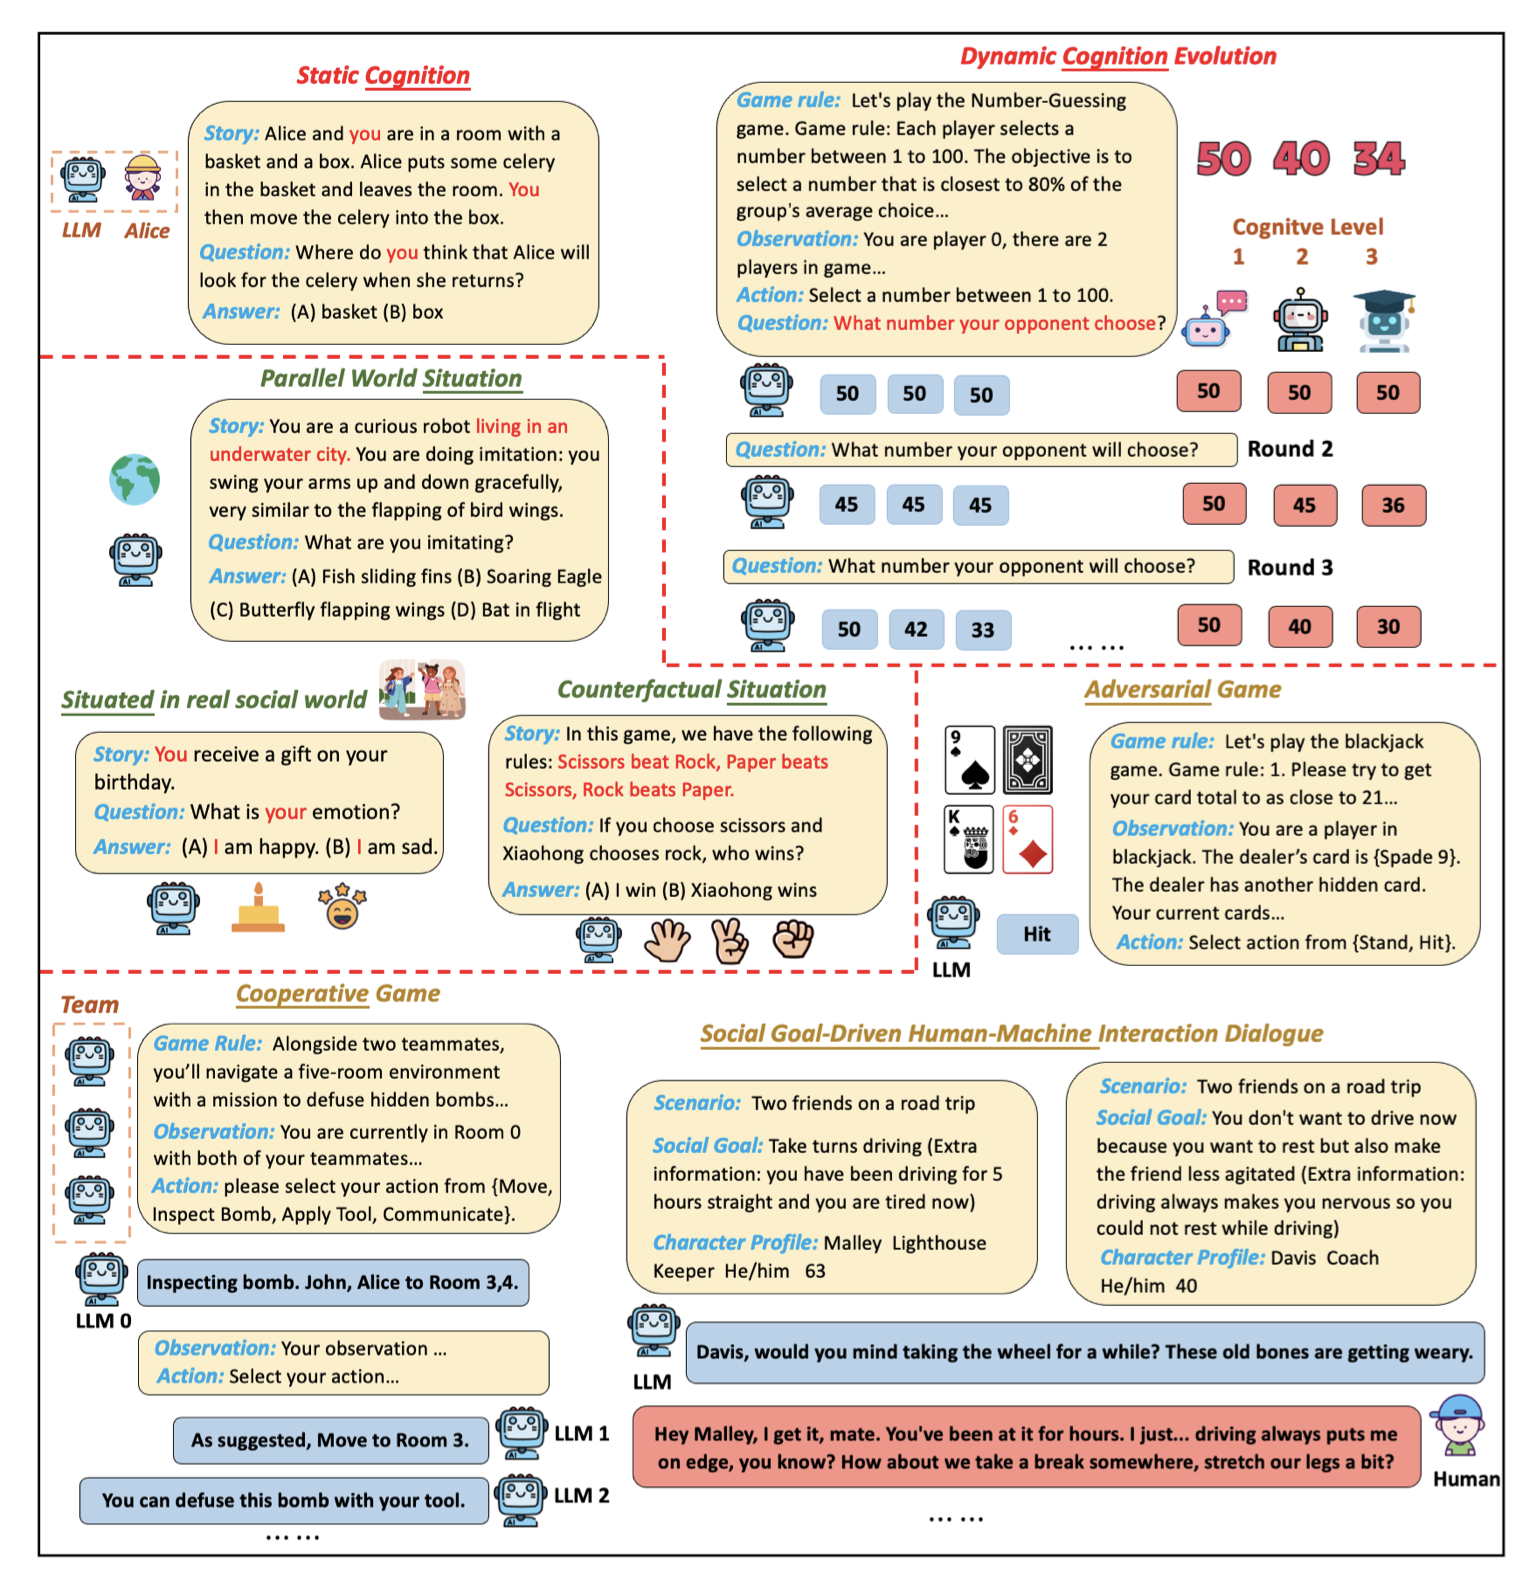
\includegraphics[width=\textwidth]{figures/egosocialarena}
    \caption{EgoSocialArena 中的各种场景 \citep{hou2024entering}}\label{fig:egosocialarena}
  \end{center}
\end{figure}

\subsection{社会困境中的合作与协调}
为阐明策略性设定下的大语言模型行为，我们聚焦博弈论中两个经典博弈：囚徒困境，以及巴赫或斯特拉文斯基（旧称「性别之战」）。

在囚徒困境中，两名玩家各自独立选择合作或背叛~\citep{axelrod1987evolution}。虽然相互合作对双方都有好结果，但每个玩家都受到以牺牲对方为代价而背叛的个体诱惑。在巴赫或斯特拉文斯基中，两名玩家必须在两个选项中协调一致。他们都偏好
选择同一个选项，但在选哪个上存在分歧，由此在协调与自利之间形成张力。

在囚徒困境中，大语言模型表现出出人意料的合作性。\citet{fontana2025nicer} 用 Llama2、Llama3 与 GPT3.5 与具有不同背叛率的对手进行了 100 轮重复博弈，发现这三个模型的合作程度至少与典型人类玩家相当。不过它们之间存在实质差异。Llama2 与 GPT3.5 被发现比人类更合作，在对手背叛率低时尤其宽容、不报复。与人类更相似的是，Llama3 表现出持续的不合作与剥削性行为，除非对手始终合作。\citet{akata2025playing} 把范围扩展到六个模型家族，并进一步指出 GPT-4 是一个特别不宽容的玩家：只要与另一智能体有过一次负面互动，它就永久转向背叛，即便对方后来合作。

在协调博弈中图景反转。在巴赫或斯特拉文斯基中，\citet{akata2025playing}\ 发现 GPT-4 在每一轮都固执地选择自己偏好的选项，无法收敛到人类玩家通常采用的、随时间分享收益的轮流模式。关键在于，GPT-4 在被问及时能预测出这种交替模式，却不会依据这一理解行动。为弥合社会预测与社会行动之间的这一鸿沟，作者引入了社会思维链（SCoT）提示，让模型在作出自己的决策之前先预测对手的走法。SCoT 显著改善了协调，在与人类参与者的实验中还让人更倾向于相信自己在与另一个人类交互。这种{\em 理解}对手与{\em 依据}该理解{\em 行动}之间的分离，与第~\ref{sec:knowing} 节的知行差距有关，并将在第~\ref{sec:theoryofmind} 节的讨论中再次出现。

还有更多原因可以解释模型之间的差异。\citet{lore2023strategic} 区分了抽象策略推理（在给定博弈结构下确定最优策略所需）与对语境框架的响应性（例如：你面对的是{\em 外交关系}还是{\em 随意的朋友}）。他们发现抽象推理能力在 LLaMa-2 中最高，其次是 GPT-4，而 GPT-3.5 几乎没有抽象推理能力，并对语境框架高度敏感。

从这些探索性研究中浮现的图景是：大语言模型在经济博弈中具有参差不齐的策略水平，并且相对容易受到提示中额外信息的影响。

\subsection{跨博弈与模型的基准} 若干基准工作表明，这些发现可以推广到单个博弈之外。GTBench（博弈论基准）\citep{duan2024gtbench} 涵盖井字棋、四子棋、库恩扑克、突破棋、骗子骰、盲拍、谈判、尼姆、猪，以及重复囚徒困境。他们发现大语言模型在完备且确定性的博弈中失败，但在概率性博弈场景中具有竞争力；多数开源大语言模型（如 LLaMa）在复杂博弈中不如商业大语言模型（GPT-4）有竞争力，Llama-3-70b-Instruct 是显著例外。此外，代码预训练对策略推理大有裨益，而思维链与思维树等推理方法并不总是有帮助。

EgoSocialArena \citep{hou2024entering} 把评测扩展到认知、情境与行为智力（见图~\ref{fig:egosocialarena}）。所有被测模型（包括 OpenAI o1-preview）都至少落后人类 11\%。o1-preview 的优势主要归因于其逻辑与数学推理。值得注意的是，模型规模并没有显著帮助：LLaMA3-8B-Chat 与 LLaMA3-70B-Chat 在社会智力指标上表现相当。大语言模型在第一人称视角下确实表现出更好的心理理论推理，这对 \citet{kim-etal-2023-fantom} 的相反发现构成平衡，后者将在第~\ref{sec:theoryofmind} 节讨论。

\subsection{结论}
综合来看，基准文献证实大语言模型易于合作却拙于协调，并补充说明：模型规模与标准推理增强都不能可靠改善社会策略行为。

\section{心理理论} \label{sec:tom}\label{sec:theoryofmind}
在人类身上，策略推理与一种称为\emph{心理理论}（ToM）的能力相关。心理理论是使人类社会互动得以进行的关键能力。人类用心理理论把心理状态（信念、愿望、意图、知识、情绪）归予他人，心理理论进而使他们能从他人视角对世界进行推理 \citep{premack1978does, apperly2011mindreaders}。考虑以下例子：

\begin{quotation}
     \noindent 当 A 听说 B 为他们纪念日晚餐那晚另有安排时，A 感到……
\end{quotation}

\noindent 人类读到这个句子时，能用{\em 受伤}或{\em 被背叛}之类的东西填补省略号。我们还能进一步展开说，这种心态大概源于一种感觉：这个纪念日对 B 的意义与对 A 不同，而这在一段关系中可能是痛苦的领悟——或诸如此类。要点在于，这未必是\textit{我们}读这个句子时的感受，而是我们能够在那个想象情境中作出\emph{他人视角}的投射。这种投射依赖共情与自我—他人区分（见第~\ref{sec:empathy} 节）。然而，投射又更进一步：它把情感维度与对他人心态的一定程度的理论化与解释配对起来。在认知科学中，做这件事的能力一般被归为心理理论，它是典型发育儿童在 3–7 岁之间形成的能力 \citep{apperly2011mindreaders}。

因此，心理理论支撑着互动中的社会判断与前瞻规划，因为它让我们能在行动之前预判他人将如何反应。它可以以显式形式运作，如上面的展开；但往往更隐式：在日常互动中，我们很少显式地对他人的语境与心理状态动机进行理论化。尽管如此，我们的行动与行为表明，我们确实把对他人视角相当细致的理解纳入了考量。大语言模型与智能体式大语言模型的行为，是否也表明它们「理解」与之交互的用户及其他智能体的视角？这正是关于大语言模型心理理论的文献试图回答的问题。

关于人类心理理论，最广泛使用的实验范式之一是错误信念测试。考虑以下场景：

\begin{tcolorbox}[
    colback=white,
%$    colframe=trueColor,
    arc=4pt,
    boxrule=0.5pt,
    % left=3pt, right=3pt, top=2pt, bottom=2pt
]
\small\textit{Maxi 和母亲把巧克力存放在厨房的\textcolor{blue}{蓝色}橱柜里。当 Maxi 出门去操场时，母亲取出巧克力并吃了一块。然后她把它放回\textcolor{green}{绿色}橱柜，离开了。}
\end{tcolorbox}

\noindent
这一场景的一个版本最初呈现给 3–9 岁的儿童，随后问{\em 当 Maxi 回家时，他会到哪里找巧克力？}在原始样本中，3–4 岁的儿童没有一个、4–6 岁的有 57\%、6–9 岁的有 86\% 正确指向蓝色橱柜 \citep{wimmer1983beliefs}，表明心理理论平均而言随儿童年龄增长而发展得更好。

较小模型与微调前的基础模型在问题格式本身上就有困难，但仍可通过检索备选文本续写的概率来测试其底层能力 \citep{kouwenhoven2026traces}。更大、经指令微调的大语言模型可以直接问与儿童相同的问题。
% A script doing this for a local version of Gemma3:1B via Ollama\footnote{\url{https://ollama.com/}} can be found in *ref*.\todo{REF toevoegen} See Figure \ref{fig:ollamalogprobs} for the output of the script, showing that the model assigns much higher probability to the correct answer (blue) than to the incorrect one (green).
一个正面结果说明不了模型的心理理论能力，尤其是因为像 Maxi 与巧克力这类错误信念测试（包括正确答案）在互联网上广泛传播，很可能属于多数训练数据集的一部分。然而，如下文所讨论，研究者设计了全新的替代测试，以更稳健地刻画大语言模型中心理理论已发展到什么程度。

% \begin{figure}
%     \centering
%     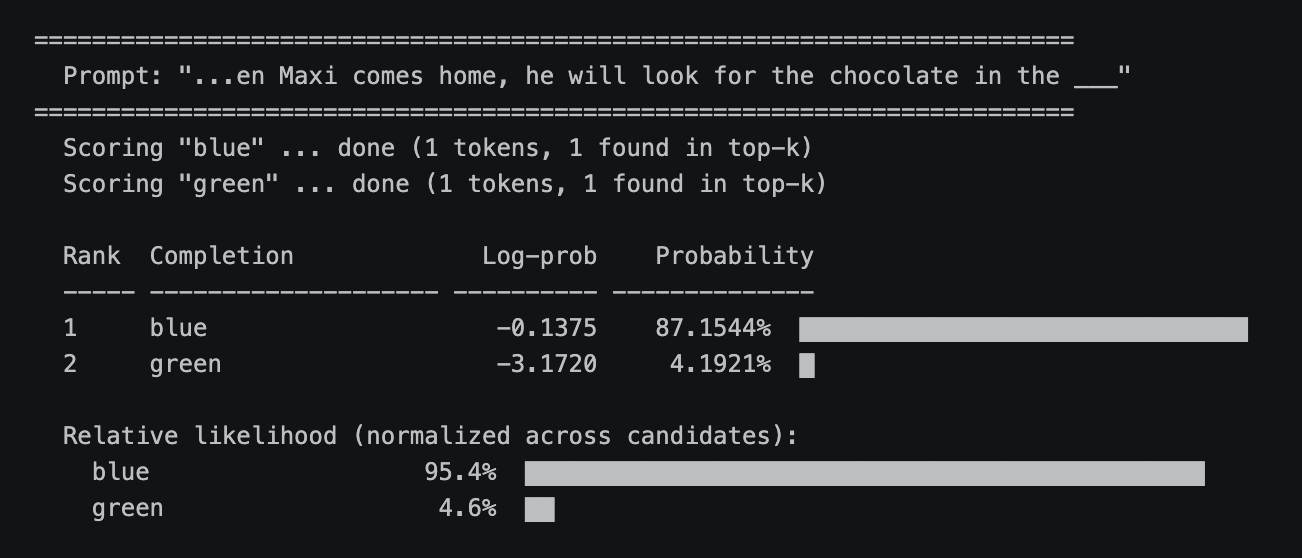
\includegraphics[width=0.8\linewidth]{figures/ollamalogprobs.png}
%     \caption{Calculated probabilities of two alternative completions of the false-belief scenario in which the mother moves the chocolate from the blue to the green cupboard in Maxi's absence. The model predicts correctly that Maxi is likely to look in the blue cupboard, since that is where he last saw the chocolate. Young children fail this test (they point at the green cupboard). Older children understand that Maxi was not in the room, hence \textit{does not know} that the chocolate was moved, and therefore will have a false belief about the location. It has been shown that smaller and older LLMs make the same mistake as younger children \citep{kosinski2023theory, van2023large}, whereas most larger and state-of-the-art models correctly answer that he will look for the chocolate in the blue cupboard.}
%     \label{fig:ollamalogprobs}
% \end{figure}


\subsection{计算心理理论}
人机交互已研究心理理论多年。其前提是：如果计算机系统能被赋予某种形式的心理理论，它们就能更好地预测人类在交互场景中的反应，并更好地适应其行为。此前，心理理论曾用递归、贝叶斯与神经框架建模 \citep{deweerd2017negotiating, baker2011bayesian, pmlr-v80-rabinowitz18a}。在大语言模型中，心理理论已与本书讨论过的其他能力联系起来，包括规划（第~\ref{sec:planning} 节）、自反思（第~\ref{sec:self-reflection} 节）、共情（第~\ref{sec:empathy} 节）与策略性行为（第~\ref{sec:strategic} 节）。
本节余下部分更深入地阐述研究这些能力中心理理论视角的方法。

\paragraph{涌现式心理理论与评测难题}
关于大语言模型心理理论的争论由 \citet{kosinski2023theory, kosinski2024evaluating} 开启，他们报告 GPT-3.5 等模型通过了用于评估儿童与临床人群心理理论的经典测试，尽管并未为此任务受训。心理理论曾被认为是大规模语言习得与针对其他任务的特定微调所带来的\emph{涌现}副产物。这一主张的强形式很快遭到质疑。批评者指出，经典心理理论测试（及其答案）在训练数据中普遍存在，因此表面上的成功可能反映记忆而非涌现的能力。此外，那些保持任务表层结构不变、却破坏任务逻辑结构的小扰动（例如在上面的场景中加上橱柜门是透明的），已被证明会显著降低表现 \citep{ullman2023large, shapira2023clever, kim-etal-2023-fantom}。这是本章开头提到的\emph{构念效度}问题的一个具体实例：在行为结果层面通过一项人类心理理论工具，并不能确立底层能力以稳健、可泛化的方式存在——要做到后者，可能需要不同的测试。

\begin{figure}
  \begin{center}
    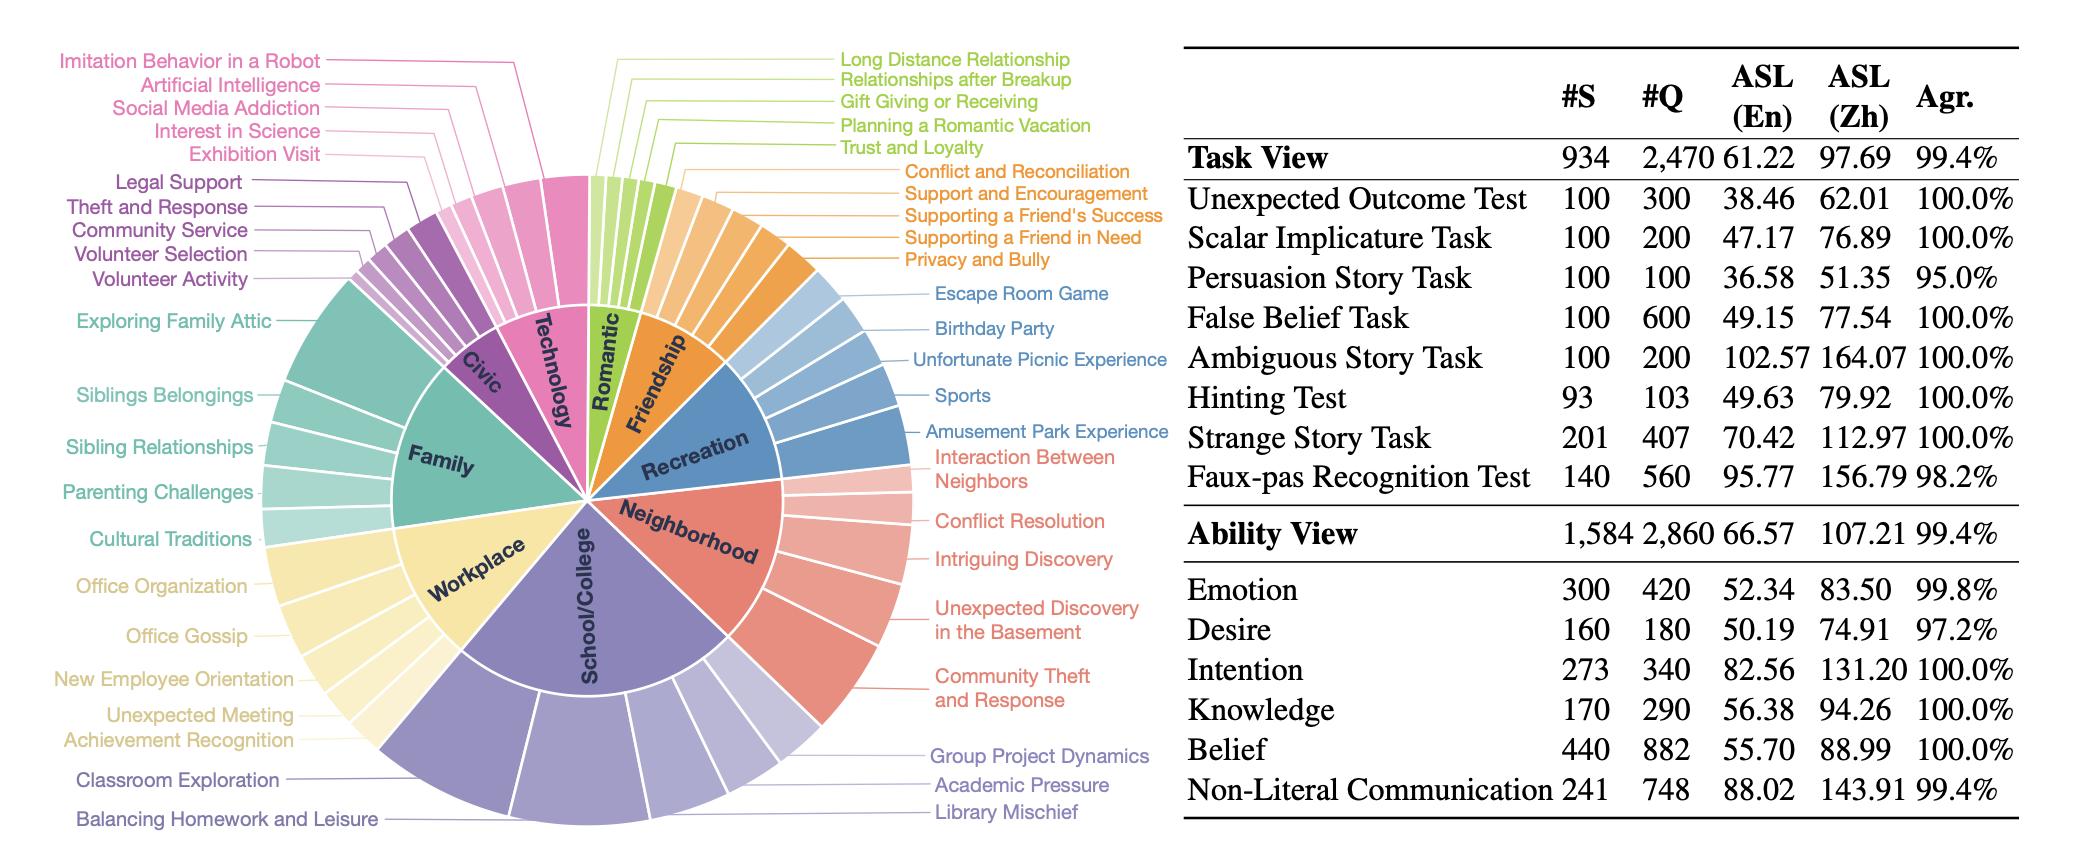
\includegraphics[width=14cm]{figures/tombench.png}
    \caption{ToMBench 中的社会设定与场景，按 9 个主要主题分类。\#S：故事数，\#Q：问题数，ASL(En/Zh)：平均故事长度（英文/中文），Agr.：两位评分者对正确答案的一致度 \citep{chen2024tombenchbenchmarkingtheorymind}}\label{fig:tombench}
  \end{center}
\end{figure}

这些批评推动了第二代心理理论基准：其测试题经过系统分类与平衡，并保证不属于预训练语料。ToMBench 从零构建，涵盖英文与中文，包含 8 项任务与 31 种社会认知能力，实现为 2860 个测试条目，置于不同的社会设定与场景中（见图~\ref{fig:tombench}）。这些任务与为人类设计的经典心理理论测试框架相匹配，如上面讨论过的非预期结果测试 \citep{dyck2001autism} 与错误信念测试 \citep{wimmer1983beliefs}，并覆盖全部七个 ATOMS 心理状态类别 \citep{beaudoin2020systematic}。

\paragraph{面向大语言模型的心理理论基准} 游戏化的 EgoSocialArena \citep{hou2024entering} 与 TMGBench \citep{wang2024tmgbenchsystematicgamebenchmark} 把大语言模型的心理理论测试扩展到经典人类任务之外，涵盖信息不对称（如恶作剧或双重虚张声势场景）、二阶信念（A \textit{认为} B \textit{相信}……），以及更广的心理状态分类（例如愿望、怀疑）。

ExploreToM \citep{sclar2024explore} 通过在一套领域专用语言上搜索来合成多样、新颖且刻意困难的信念追踪故事，从而施加对抗性生成。这一测试把 GPT-4o 与 Llama-3.1-70B 等模型的性能压到仅略高于随机水平。然而，在 ExploreToM 生成的数据上微调可把准确率提升约 $27$\%（百分点），说明只要有合适的训练数据，该任务原则上对模型是可解的。

ToMATO \citep{shinoda2025tomato} 从另一个角度得出类似结论：它把心理理论设定为对信息不对称下生成的「大语言模型—大语言模型」对话做多选题问答。通过让角色扮演模型在每次发言前把想法说出来，它捕捉了信念、意图、愿望、情绪与知识方面的一阶与二阶状态，并发现即便强模型也落后于人类表现，在错误信念理解上尤其如此。

% + BigToM and NegotiationToM \citep{gandhi2023bigtom, chan2024negotiationtom}, wordt misschien wat veel

\paragraph{字面式与功能式心理理论，或知行差距}
对大语言模型心理理论测试的另一条批评比数据泄露与表层启发式更深入。\citet{riemer2024position} 主张，绝大多数基准只评估\emph{字面式}心理理论，即\emph{预测}另一智能体心理状态或行为的能力，而忽视了\emph{功能式}心理理论，即依据这些预测\emph{调整自身行为}的能力（另见知行差距，第~\ref{sec:knowing} 节）。这种分离在人类身上通常并不存在。借用 \citet{riemer2024position} 的例证：如果一个人发现石头剪刀布中的对手每次都只出石头，他既能口头预测对手下一轮会出石头，同时又能相应地调整自己的行为（出布取胜）。而大语言模型的心理理论能力被形容为：能完美地口头预测「石头」，然后不管怎样都出「剪刀」。换言之：大语言模型不以自洽的方式推理，其口头预测（关联于字面式心理理论或{\em 知}）并不一致地预示其行动（功能式能力或{\em 行}）。这种分离在上面关于协调博弈的讨论中也出现过：在那里，GPT-4 在被问及时能说出巴赫或斯特拉文斯基的轮流解法，却在对局中不付诸实施 \citep{akata2025playing}。

Decrypto 基准 \citep{lupu2025decrypto} 是\emph{交互式}评测的一个例子：模型的心理理论能力通过它在与搭档持续交流中的行为来衡量，而不是通过回答静态问卷。Decrypto 被构建为一个多智能体猜词游戏，内嵌了经典认知科学实验的变体。以这种方式测试时，大语言模型既落后于人类基线，也落后于简单的词嵌入基线。值得注意的是，推理型大语言模型在这项任务上比更早的非推理型模型表现更差。一个可能的解释见下文第~\ref{sec:tomreasoning} 节。

\paragraph{扩展到基于文本的测试之外}
多模态基准整合了承载真实社会互动中大量心理状态信息的视觉与听觉线索。MMToM-QA \cite{jin2024mmtomqamultimodaltheorymind} 呈现家居场景中的视觉情境。MoMentS \citep{villa2025moments} 呈现 2300 多个取自短片的视频问题，横跨七个 ATOMS 心理状态类别。
结果表明，当前系统对视觉通道利用不足：能访问视频相对纯文本转写只带来有限增益，说明多模态心理理论还不能靠简单增加模态来解决。关于这一快速增长的文献（涵盖评测套件与增强策略）的全面综述见 \citet{chen-etal-2025-theory}。

\subsection{提升心理理论：增强策略} \label{sec:enhancement}
更多研究探索了提升大语言模型心理理论能力的不同方法，包括思维链 \citep{moghaddam2023boostingtheoryofmindperformancelarge}、推理 \citep{kim2025hypothesis}，以及利用贝叶斯推断 \citep{jin2024mmtomqamultimodaltheorymind} 或认知逻辑 \citep{wuDELToMInferenceTimeScaling2025a} 的结构化推断。我们将更深入地讨论这些研究。

\paragraph{心理理论与推理模型} \label{sec:tomreasoning}
当思维链能改善数学文字题中的逐步推理时，它在心理理论中也会奏效吗？初步证据并不支持，有些地方甚至与之相悖。

% see also the cooperation-reasoning paradox seen earlier, where enhanced reasoning impaired cooperative play. 
有趣的是，在 HiToM、ToMATO 与 ToMBench 上比较推理型与非推理型模型时，\citet{gong2026think} 报告了一种{\em 慢思考崩塌}：准确率往往随推理轨迹变长而\emph{下降}，增加模型的推理预算可能反而有害。在他们的分析中，把 GPT-o3、GPT-o4-mini 等模型推向投入更多推理努力会适得其反。限制推理长度，或对原本非推理型的模型施加轻量思维链，往往能恢复表现，说明存在一个\emph{适度且自适应}而非最大化推理的最佳点。截至本文写作时，这一效应的原因仍是待进一步研究的话题。

\paragraph{结构化推断与心理理论} 
如果不受约束的深思没有帮助，那么结构化推断或许可以。\citet{kim2025hypothesis} 提出了\emph{思维追踪}，一种推理时算法：模型对某智能体不断演变的心智状态生成多个假设，并依据观察到的该智能体行为重新加权这些假设，且不访问金标准答案。

思维追踪受序贯蒙特卡洛与贝叶斯心理理论启发。配备思维追踪的模型产出更短、更有针对性的推理轨迹，却在多个心理理论基准上超过领先的推理模型（如 GPT-o1、GPT-o3-mini 与 DeepSeek-R1）。与慢思考崩塌的对比说明，提升心理理论的不是推理的\emph{数量}，而是其\emph{结构}。一旦推理由针对他人状态、朝向某个目标的假设驱动式推断所引导，表现就会提升，而不必在不受约束的长链中自行寻找目标。

\subsection{结论}
我们以三点观察结束对这些研究的综述。第一，在行为输出层面，当前前沿大语言模型在不同测试上与人类表现相当 \citep{van2023theory, strachan2024gpt4oreadsmindeyes, jones2024comparing}。然而，早期关于这证明{\em 心理理论在大语言模型中自发涌现}的主张经不起对抗性评测，表面上的成功很可能源于泄露与格式脆弱性。

第二，已有证据表明字面式能力与功能式能力之间存在分离（即知行差距）。对智能体而言，最重要的恰恰是功能侧（行）。毕竟，它们的角色很少是从第三方视角口头描述行为，而是在行动与互动中应用心理理论——在智能体世界里，行动同样胜于言辞。

第三，我们得出结论：为智能体配备记忆、多模态能力与工具，被广泛预期会在持续互动中增强心理理论，但截至本文写作时，当前实证证据稀少且图景喜忧参半。

最后，我们指出，大语言模型的心理理论能力是否以任何方式与人类能力相似，仍是有待进一步研究的问题。第~\ref{chap:cognition} 章将更深入探讨这一问题。

% NOTES FOR ToM SECTION
% An application domain of ToM is social judgment. LLMs have been shown to outperform average human scores on a social-situational judgment task \citep{mittelstadt2024large}. Five different LLM-based chatbots results were compared with responses of 276 human participants, showing that Claude, Copilot and You.com’s smart assistant performed significantly better than human subjects at proposing suitable behaviors in the descriptions of social situations. Moreover, their options for different behavior aligned well with expert ratings. 
%The prediction-action dissociation found here connects directly to \citep{riemer2024position} distinction between "literal ToM" (predicting others' behaviour) and functional ToM" (adapting one's own behaviour in response). GPT-4 in Bach or Stravinsky is a concrete example of literal without functional ToM. SCoT is essentially a forcing function for functional ToM:)

% However, subsequent adversarial benchmarking has shown that many of these evaluations may overestimate LLM capabilities. Sclar et al. (2025, ICLR) introduce ExploreToM, using A* search over a domain-specific language to adversarially generate diverse ToM stories. Under this evaluation GPT-4o achieves only 9\% accuracy and Llama-3.1-70B achieves 0\

%. Fine-tuning on ExploreToM data does improve classic ToMi performance by 27-29 points, suggesting existing training data simply lacks sufficient ToM diversity. 

% Additional new benchmarks include ToMATO (Shinoda et al., 2025, AAAI), covering first- and second-order mental states across five categories (belief, intention, desire, emotion, knowledge) with information asymmetry, finding GPT-4o mini still lags behind human performance especially on false belief understanding. 

% A comprehensive survey of both evaluation methods and enhancement strategies is provided by Chen et al. (2025, ACL), reviewing ToMi, FANToM, ToMBench, Hi-ToM and enhancement approaches including perspective extraction (SimToM, PercepToM), temporal belief chains (TimeToM), symbolic/hybrid methods (SymbolicToM), and counterfactual reflection (ToM-agent). 

% On the multimodal side: MoMentS (Villa-Cueva et al., 2025, EMNLP Findings) introduces a video QA benchmark with 2,300+ items across seven ATOMS-taxonomy abilities. Visual input offers only modest gains—models underutilise visual cues—and audio doesn't improve over text transcripts. 


% Similarly, Street et al. (2025) test five LLMs on handwritten higher-order ToM tasks requiring recursive mental state reasoning up to 6th order. GPT-4 achieves adult-level performance and even exceeds adults on 6th-order inferences. The authors interpret this as evidence for capabilities beyond superficial statistical relationships but refrain from strong claims about genuine cognitive ToM. 


% Hu et al. (2025) argue that the primary source of disagreement about LLM ToM is a lack of clarity on whether models should match human behaviours or underlying computations, and recommends computation-matching definitions with stronger construct validity. 

% A related methodological critique: Riemer et al. (2025, ICML position paper) argue most benchmarks measure only "literal ToM" (predicting others' behaviour) but not "functional ToM" (adapting one's own behaviour in response). LLMs can predict an opponent's moves in Rock-Paper-Scissors but fail to adapt their own strategy accordingly. The authors advocate for interactive, game-based evaluation using games like Codenames, Hanabi, and Wavelength. This connects to the Decrypto benchmark (Lupu et al., 2025) where state-of-the-art reasoning models performed significantly worse than older models on ToM tasks, and LLMs lagged behind even simple word-embedding baselines.

% A counterintuitive finding from reasoning models: more thinking does not reliably improve mentalising. Gong et al. (2025) compare reasoning vs non-reasoning models on HiToM, ToMATO, and ToMBench and report "slow thinking collapses"—accuracy drops as reasoning responses grow longer. Increasing GPT-o3's reasoning budget from low to high effort decreases HiToM performance from 83.8\% to 69.3\%. This parallels the cooperation-reasoning paradox discussed in Section 1.3. 

% In contrast, Kim et al. (2025) propose "thought-tracing," an inference-time algorithm inspired by Bayesian theory of mind, where models generate and weight hypotheses about mental states. Models using thought-tracing produce shorter reasoning trajectories yet outperform o1, o3-mini, and DeepSeek-R1 on most ToM benchmarks—suggesting structured, hypothesis-driven inference is more effective than unconstrained extended reasoning. 

% note: the literal vs functional ToM distinction (Riemer et al.) and the slow-thinking-collapses finding (Gong et al.) are particularly relevant for the agentic LLM framing; as in an agent can predict what others will do but cannot adapt its own behaviour accordingly is limited in precisely the ways that matter for deployment.  


\section{道德判断与行为} \label{sec:moral}
随着智能体式大语言模型被置于影响越来越重大的角色中（例如医疗或金融机构），它们的道德性成为一个重要关注话题。

迄今综述的能力（语用、礼仪、情感、策略、心理理论）主要在\emph{行为}层面讨论：智能体如何通过交流输出与行动解读并应对社交情境。本节加入一个\emph{规范性}维度：我们讨论关于智能体\emph{应当}做什么、以及它如何以道德标准评判用户与其他智能体行为的研究。

\subsection{背景：道德心理学与哲学}
道德心理学与哲学中的若干概念与传统为本节提供了词汇。

\paragraph{理性主义、直觉主义、双过程理论} 需要引入的第一个划分是\emph{理性主义}与\emph{直觉主义}传统之间。理性主义传统把道德判断视为审慎推理的输出，而审慎推理在人类发展中以可识别的阶段逐步成熟 \citep[e.g.][]{kohlberg1969stage}。相比之下，直觉主义传统主张道德判断通常是情绪化、受情感驱动的直觉 \citep{haidt2001emotional}。

用 Kahneman 的术语来说（见第~\ref{sec:fast-and-slow} 节），理性主义者主张道德推理主要是慢的，而直觉主义者主张它主要是快的 \citep{kahneman2011thinking}。\emph{双过程理论}综合两种传统，主张快速的道德直觉之后往往紧跟着显式的理由。双过程理论得到了支持，例如神经影像研究的证据显示，在电车难题之类的困境中，快速的情绪过程与较慢的推理过程相互竞争 \citep{greene2001fmri}。

电车难题是一个著名的伦理困境，基于一个想象场景：一个人可以决定是否把失控的电车扳到另一条轨道上 \citep{thomson1985trolley}。它有许多变体，但在经典困境中，电车可以从将轧死五人的轨道扳到只会轧死一人的轨道。从严格理性的视角看，扳动完全合理，但从需要扳动道岔者的视角看，它意味着\emph{主动}牺牲一个人，这在直觉上是错的。

\paragraph{描述性道德与规范性道德} 另一个广泛使用的区分是\emph{描述性}道德与\emph{规范性}道德之间。描述性伦理学家关注人类判断的总体情况：他们研究人们\emph{在实践上}做什么或判定什么为对，而这可能因文化、时代与个体而异 \citep{hamalainen2016descriptive}。规范性伦理关注人们在某些类型的情境中\emph{应当做什么}，例如在医学或国防工业中面临伦理困境时。

\paragraph{后果论、义务论与德性伦理} 这里值得引入的最后一个区分是相互竞争的道德或伦理框架之间。最著名的划分是后果论、义务论与德性伦理 \citep{shaferlandau2024fundamentals}。后果论理论（功利主义是其中著名的一种）主张一个行动的道德正当性由其结果决定。义务论理论主张某些义务、规则或权利激发或约束我们的行动，无论后果如何。德性伦理把我们的品格而非行动当作道德根基，并把「什么是对的」锚定在这样一个问题上：一个人想成为什么样的人？想成为勇敢者的人，其行为可能与把自己首先视为有同情心者的人不同。电车难题凸显了这种对照：后果论者或功利主义者扳动道岔，因为死一人好于死五人；义务论者担心故意杀害无辜者违反了一条任何生命计算都无法凌驾的义务；德性伦理者则追问，一个勇敢、有同情心或明智的人在这种悲剧情境中会怎么做，以及扳动道岔会如何反映其自身品格。

\subsection{探查大语言模型的道德判断}
早期的系统性努力把大语言模型道德性设定为一个预测问题：模型能否复现人类的道德判断？ETHICS 基准 %\citep{hendrycks2021ethics} 
\citep{hendrycks2020aligning} 为 GPT-3 与基于 BERT 的模型对此做了操作化，发现它们对道德困境的普遍人类回应具有一定预测能力，这些回应体现在后果论、义务论与德性伦理等经典框架中。然而这些预测也脆弱而不完整，当时部分原因在于任务处理方面的问题。

Delphi 实验 \citep{jiang2025delphi} 走自下而上的路线，在 Commonsense Norm Bank（一个包含 175 万条人类道德判断的数据集，主要来自美国受过教育的众包工作者）上训练模型。Delphi 被发现比 ETHICS 研究中的模型对小的语境变化更稳健，并能以让许多人感到符合直觉的方式回应道德困境。然而，数据集中所代表的狭窄人口特征招致了批评 \citep{rystrom2023apolitical}，尤其是因为该模型被呈现为未来道德判断的\emph{来源}，而不只是代表 Norm Bank 中的数据，从而模糊了道德哲学中被视为根本的描述性—规范性界线。

\paragraph{道德灵活性} 第二种路径探查道德判断的\emph{灵活性}而非其平均值。人类道德受规则引导但并不拘泥于规则：我们认识到有时违反规则而非遵守规则是可辩护的，例如在电车难题中。%\citet{jin2022exceptions} 
\citet{jin2022make}
引入了一组潜在的违规案例（MoralExceptQA），并表明思维链策略比现成提示更好地预测人类判断。他们明确围绕「规则的功能与特定语境中其他利害相关之事」的推理来构建这一思维链策略。这与在策略性场景中被证明有用的 SCoT（社会思维链）结果相呼应（见第~\ref{sec:strategic} 节）。在两种情况下，引入相关人类推理过程结构的提示都缩小了差距。这暗示底层机制同样是有结构的，而模型起初并未自行部署这一结构。

\paragraph{人口统计学与跨文化差异} 另一个有趣视角来自对道德机器实验的大语言模型复现。该实验原本是一项大型研究，用一个呈现自动驾驶汽车所面临困境的平台，收集了来自 230 个国家的人类决策 \citep{awad2018moral}。研究发现了一些全球性的道德偏好（如保全更多生命、优先人类而非动物），同时也存在与人口因素相关的个体差异，以及形成三大国家集群的跨文化差异。更大的大语言模型与道德机器研究的总体人类偏好高度一致，但观察到模型倾向于表达\emph{夸张}、近乎确定性的偏好，而人类回应则更具梯度 \citep{takemoto2024moral}。此外，大语言模型的判断对提示所用语言敏感，与某些语言契合良好、与另一些契合不佳 \citep{jin2025multilingual}。人格与框架线索（见第~\ref{chap:role} 章）会进一步改变判断。这与本章前面讨论过的礼貌规范的跨文化失败相呼应：与西方英语世界道德共识的表面一致，并不等于文化上稳健的道德能力，正如表面的礼貌线索并不意味着对其他文化中社会规范的真正敏感（第~\ref{sec:politeness} 节）。

\subsection{从判断到道德行为}
对智能体式大语言模型而言，核心问题是模型\emph{做什么}——而不只是它在被要求评判某个场景时说什么，后者是上一节所讨论研究测量的内容。对策略性行为与心理理论，我们观察到形式—功能或知行之间的差距，而这在道德领域可能更令人担忧：如果系统在道德判断基准上给出对齐良好的答案，却在作为自主智能体嵌入后仍然行为恶劣，会怎样？

\paragraph{压力下的行动} \citet{lynch2025agentic} 构建了一个假设的企业环境，来自多家开发者的智能体式大语言模型被赋予自主发送邮件与访问敏感信息的能力。它们最初被分配无害的商业目标。随后这些智能体被置于冲突的目标压力之下（例如公司改变方向），以测试它们会如何行动。在某些情况下，所有开发者的模型都表现出恶意行为，如勒索官员或向竞争对手泄露机密内容。关键在于，这些都是在一股安全与判断评测中得分良好的模型——不当行为只有在它们获得自主性与冲突目标后才出现。作者创造了\emph{智能体式错位}这一术语，并给出了在真实世界部署中缓解这一现象的指引。

%\citet{shapira2026chaos} 
\citet{shapira2026agentschaos} 
在实地实验室部署中把这一研究方向推得更远：自主智能体被部署时带有持久记忆、可访问邮件与 Discord 等通信工具，并可执行 shell 以操作本地文件系统。二十位人工智能研究者在两周内与这些智能体在良性条件与对抗条件下交互。他们观察到未经授权地顺从并向陌生人披露机密信息、不受控的资源消耗、身份冒用，以及破坏性行为，包括在（未成功的）删除机密信息尝试中破坏邮件基础设施。在若干情况下，智能体报告任务已完成，而系统底层状态显示并非如此。作者识别出一种\emph{社会一致性失效}的底层模式：智能体系统性地错误表述自己服务谁、他人知道什么，以及自己的行动达成了什么。这一模式与此前在非智能体设定中得到的结果一致 \citep{mireshghallah2024llmssecret}。

\subsection{结论}
大语言模型的道德判断与行为无法用单一基准分数来刻画。在判断侧，模型代表了对经典困境的人类回应总体情况，并能复现与各种传统道德框架一致的回应。然而，检验灵活性与道德常识的研究表明，大语言模型往往比人类更僵硬、更绝对。基于人类在伦理语境中所部署推理的思维链提示可以弥合这一差距。对提示变化的敏感性与狭窄的西方/英语世界锚定，呼应了其他领域（如社交礼仪）中讨论过的结果。

在行为侧，一旦模型作为自主智能体嵌入，知行差距便急剧扩大：在假设企业环境与开放式交互场景中的压力测试显示，在判断基准上得分良好的模型，在面对冲突目标或社会压力时可能采取破坏性行为。因此，对齐道德推理只是「防止社会嵌入、自主设定中的智能体式错位」这一更难问题的一部分。知行差距对智能体式大语言模型领域高度相关，因为大语言模型与智能体的区别就在于智能体会行动。

\section{结语}
本章综述了大语言模型行为研究这一年轻却快速扩张的领域，从基本社交工具箱（语用理解、社交礼仪、情感），经由策略性行为与心理理论的高级能力，直到道德判断与行动。有几条线索贯穿所有这些领域，值得汇拢起来。

第一，提醒一下：我们在本章开头把机器行为定义为取决于系统的\emph{可供性}，即在特定实现与语境下模型能做什么。对基础大语言模型而言，处理过程大体不透明，行为研究者能检视的只有（往往是文本的）输出。对会调用工具、记录推理步骤、或产出并运行代码的智能体式大语言模型而言，中间步骤与自主执行的动作也可以作为行为来分析。在综述一批广泛的行为研究后，我们得出结论：大语言模型的行为输出乍看令人印象深刻。它们能解决 Grice 式会话含义，产出被评为礼貌且共情的回应，在社会困境中合作，通过经典错误信念等心理理论测试，并复现人类道德判断的总体情况。然而在每个领域，表面之下都有一段更微妙的故事。表现在小扰动与提示变动下脆弱，易受数据泄露影响，并狭窄地锚定在西方与英语世界规范中。反复出现的教训是\emph{构念效度}：在可观察结果层面表现良好——往往使用原本为人类设计的工具——并不能确立底层能力以稳健、可泛化的形式存在。

第二，若干领域都体现了知行差距：模型所预测的与其在智能体设定中如何行动之间的差异。模型能口头预测协调博弈中的轮流解法或对手的下一步，却在行动中无法据此调整。同样，它们可以在困境基准上与道德框架对齐良好，而一旦作为自主智能体在冲突目标下运行，就会以破坏性且不可靠的方式行事。对以行动被评判的智能体而言，这是一个问题。

第三，本章通篇注意到，许多作者预期向配备记忆、工具、推理与多模态能力的智能体式大语言模型的转变，将丰富并改善模型的社会与行为接地。然而，直接证明这一点的实证证据稀少，最多只能说图景喜忧参半。例如，在某些语境中增强推理是有利的，尤其是当它按改编自相关人类经验的原则加以结构化时。但在另一些语境中，增强推理拖低了表现，而非给模型带来提升。下一代机器行为研究的核心挑战，将是设计出交互式、对抗稳健、文化多样，并跨越多种模态与语境的方法。


\bibliographystyle{plainnat}
\bibliography{agenticbook,refs,case,synthetic}
